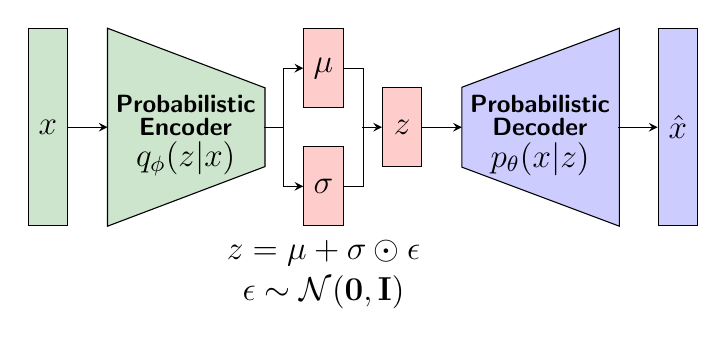
\begin{tikzpicture}
	
	
	\node[fill=Green!20, minimum width=0.5cm, minimum height=2.5cm, draw] (x) at (0,0) {\large $\boldsymbol x$};
	
	\draw[fill=Green!20] ([xshift=0.5cm]x.north east) -- ([xshift=2.5cm,yshift=0.5cm]x.east) -- ([xshift=2.5cm,yshift=-0.5cm]x.east) -- ([xshift=0.5cm]x.south east) -- cycle; 
	\node at (1.75,0.3) {{\small\sf \textbf{Probabilistic}}};
	\node at (1.75,0.0) {{\small\sf \textbf{Encoder}}};
	\node at (1.75,-0.4) {\large $q_{\boldsymbol{\phi}}(\boldsymbol{z} | \boldsymbol{x})$};
	
	\draw[-stealth] (x.east) -- ([xshift=0.5cm]x.east);
	
	\node[fill=red!20, minimum width=0.5cm, minimum height=1.0cm, draw] (mu) at (3.5cm,0.75cm) {\large $\boldsymbol{\mu}$};
	\node[fill=red!20, minimum width=0.5cm, minimum height=1.0cm, draw] (sigma) at (3.5cm,-0.75cm) {\large $\boldsymbol{\sigma}$};
	
	\node at (3.5cm,-1.6cm) {\large $\boldsymbol{z} = \boldsymbol{\mu} + \boldsymbol{\sigma} \odot \boldsymbol{\epsilon}$};
	\node at (3.5cm,-2.1cm) {\large $\boldsymbol{\epsilon} \sim \mathcal{N}(\mathbf{0}, \mathbf{I})$};
	\draw ([xshift=-0.5cm,yshift=-0.75cm]mu.west) -- ([xshift=-0.25cm,yshift=-0.75cm]mu.west);
	\draw[-stealth] ([xshift=-0.25cm,yshift=-0.75cm]mu.west) |- ([xshift=-0.25cm]mu.west) -- (mu.west);
	\draw[-stealth] ([xshift=-0.25cm,yshift=0.75cm]sigma.west) |- ([xshift=-0.25cm]sigma.west) -- (sigma.west);
	
	%\node[fill=red!20, minimum width=0.5cm, minimum height=1.0cm, draw] (z) at (5.0cm,0.0) {\large $\boldsymbol z$};
	\node[fill=red!20, minimum width=0.5cm, minimum height=1.0cm, draw] (z) at (4.5cm,0.0) {\large $\boldsymbol z$};
	\draw (mu.east) -- ([xshift=0.25cm]mu.east) |- ([xshift=-0.25cm]z.west);
	\draw (sigma.east) -- ([xshift=0.25cm]sigma.east) |- ([xshift=-0.25cm]z.west);
	\draw[-stealth] ([xshift=-0.25cm]z.west) -- (z.west);
	
	%\draw[-stealth] ([xshift=-2.5cm]z.west) -> ([xshift=-2.0cm]z.west);
	%\draw[-stealth] ([xshift=-0.5cm,yshift=-0.75cm]mu.west) -- ([xshift=-0.5cm]mu.west) |- (mu.west);
	%%%\draw[-stealth] ([xshift=-0.5cm,yshift=0.75cm]sigma.west) -- ([xshift=-0.5cm]sigma.west) |- (sigma.west);
	%%%\draw[-stealth] (mu.west) -- ([xshift=-0.5cm]mu.west) |- ([xshift=-0.5cm]sigma.west) -- (sigma.west);
	%\draw (mu.east) -- ([xshift=0.5cm]mu.east) |- ([xshift=0.5cm]sigma.east) -- (sigma.east);
	%\draw[-stealth] ([xshift=-0.45cm]z.west) -> (z.west);
	
	\draw[fill=blue!20] ([xshift=0.5cm]z.north east) -- ([xshift=2.5cm,yshift=0.75cm]z.north east) -- ([xshift=2.5cm,yshift=-0.75cm]z.south east) -- ([xshift=0.5cm]z.south east) -- cycle;
	\node at (6.25,0.3) {{\small\sf \textbf{Probabilistic}}};
	\node at (6.25,0.0) {{\small\sf \textbf{Decoder}}};
	\node at (6.25,-0.4) {\large $p_{\boldsymbol{\theta}}(\boldsymbol{x} | \boldsymbol{z})$};
	
	\node[fill=blue!20, minimum width=0.5cm, minimum height=2.5cm, draw] (xhat) at (8.0cm,0) {\large $\boldsymbol{\hat{x}}$};
	
	\draw[-stealth] (z.east) -- ([xshift=0.5cm]z.east);
	\draw[-stealth] ([xshift=-0.5cm]xhat.west) -- (xhat.west);
	
	
\end{tikzpicture}